\documentclass[11pt, a4paper]{article}
\usepackage[greek,english]{babel}
\usepackage[linesnumbered,ruled]{algorithm2e}
\usepackage{graphicx}
\usepackage[titletoc,title]{appendix}
\usepackage{float}
\graphicspath{{./img/}}
\setcounter{tocdepth}{3}
\title{\huge\textbf{Clever Support for 3D Printing}\\~\\\large CMPT464/764 ~\\Geometric Modeling in Computer Graphics~\\Course Project~\\~\\~\\~\\~\\~\\~\\\textbf{\Large Program User Manual}}
\date{~\\~\\~\\~\\~\\~\\~\\April 15, 2016}
\begin{document}
    \maketitle
    \thispagestyle{empty}
	\newpage
	\linespread{1}
	\section{File location}
	\begin{itemize}
	\item folder “models” contains the obj files for 3D models without support
	\item folder “modelsup” contains the obj files for 3D models with support provided by the author
	\item folder “result” contains the results of the program which are the obj files for 3D models with support 
	\item folder “clever\_support” contains the program after making file
	\end{itemize}

	\section{User Interface}
	\begin{figure}[H]
  		\centering
      	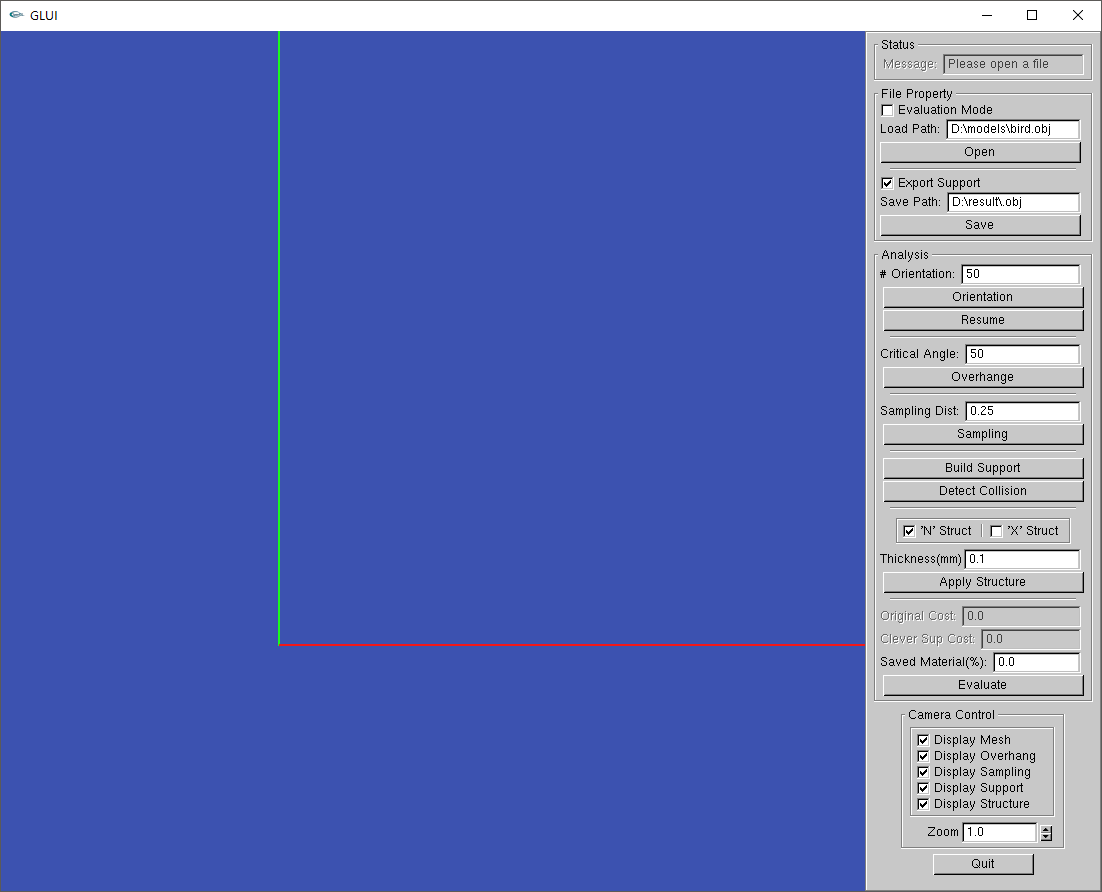
\includegraphics[width=1.0\textwidth]{UI.png}
  	\caption{\textit{The user interface is a glut window with glui controls.}}
	\end{figure}
	\section{Open/Save File(normal mode)}
	\begin{figure}[H]
  		\centering
      	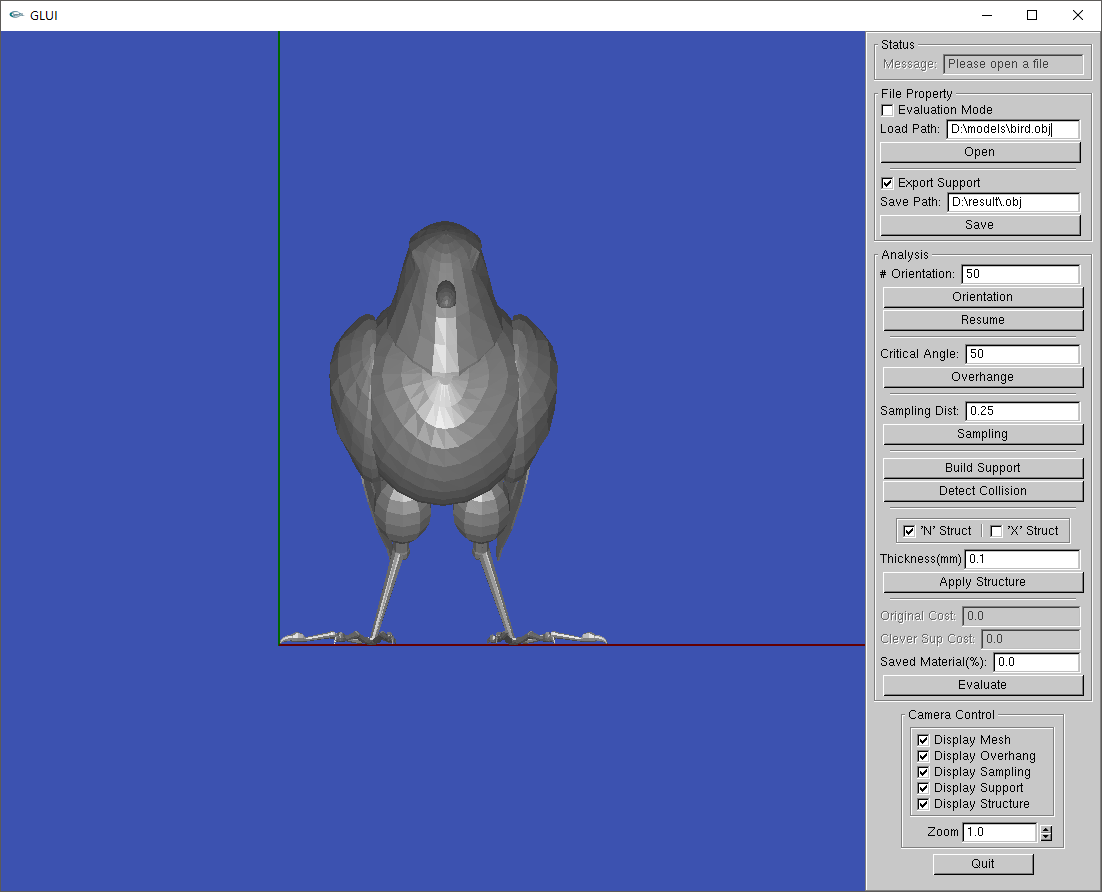
\includegraphics[width=1.0\textwidth]{open.png}
  	\caption{\textit{After inputting the correct file path, a 3D model file be opened and shown. If "Evaluation Mode" is selected, the program will enter evaluation mode. If "Export Support" is selected, the support structure will be saved along with the file.}}
	\end{figure}
	\section{Open/Save File(evaluation mode)}
	\begin{figure}[H]
  		\centering
      	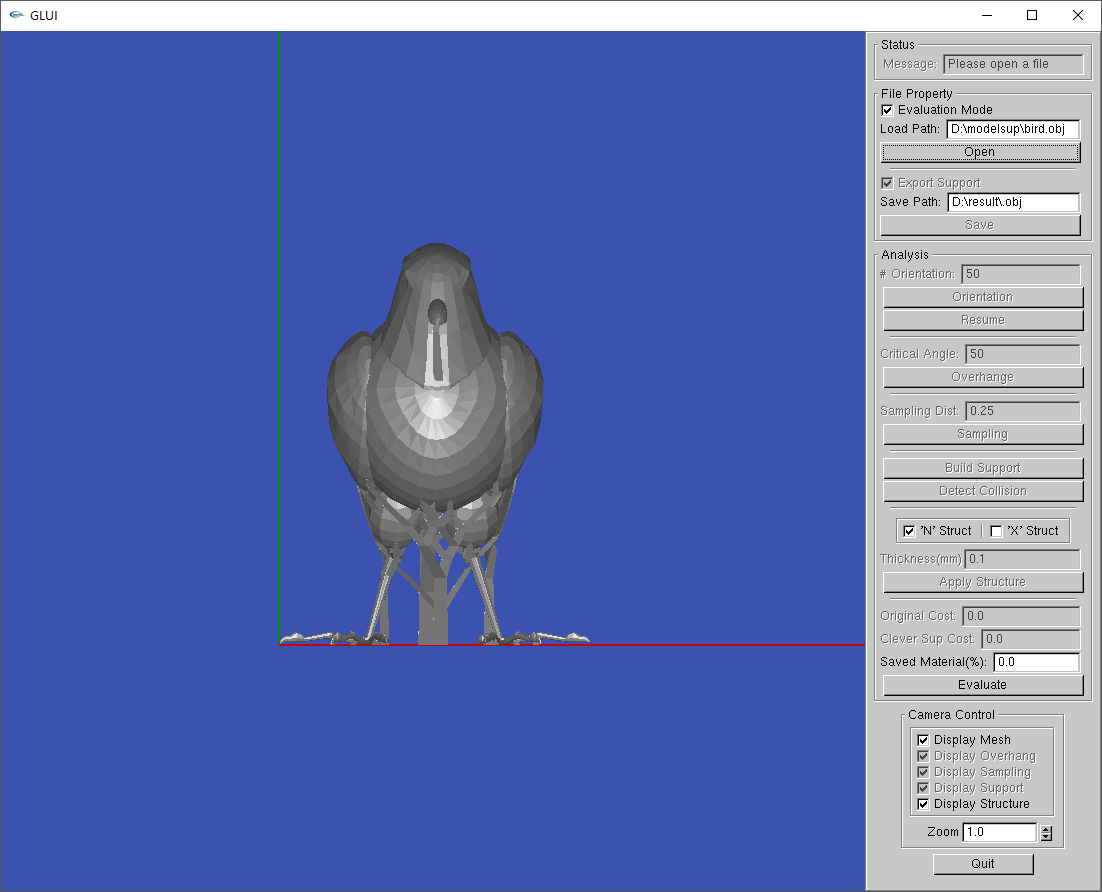
\includegraphics[width=1.0\textwidth]{emode.png}
  	\caption{\textit{The input model will be seperated into the model and its support. IN this mode, no support will be generated. Save file function will save the same file to a different place. Evaluate funciton will show the total area of the support structure faces.}}
	\end{figure}
	\section{Orientation}
	\begin{figure}[H]
  		\centering
      	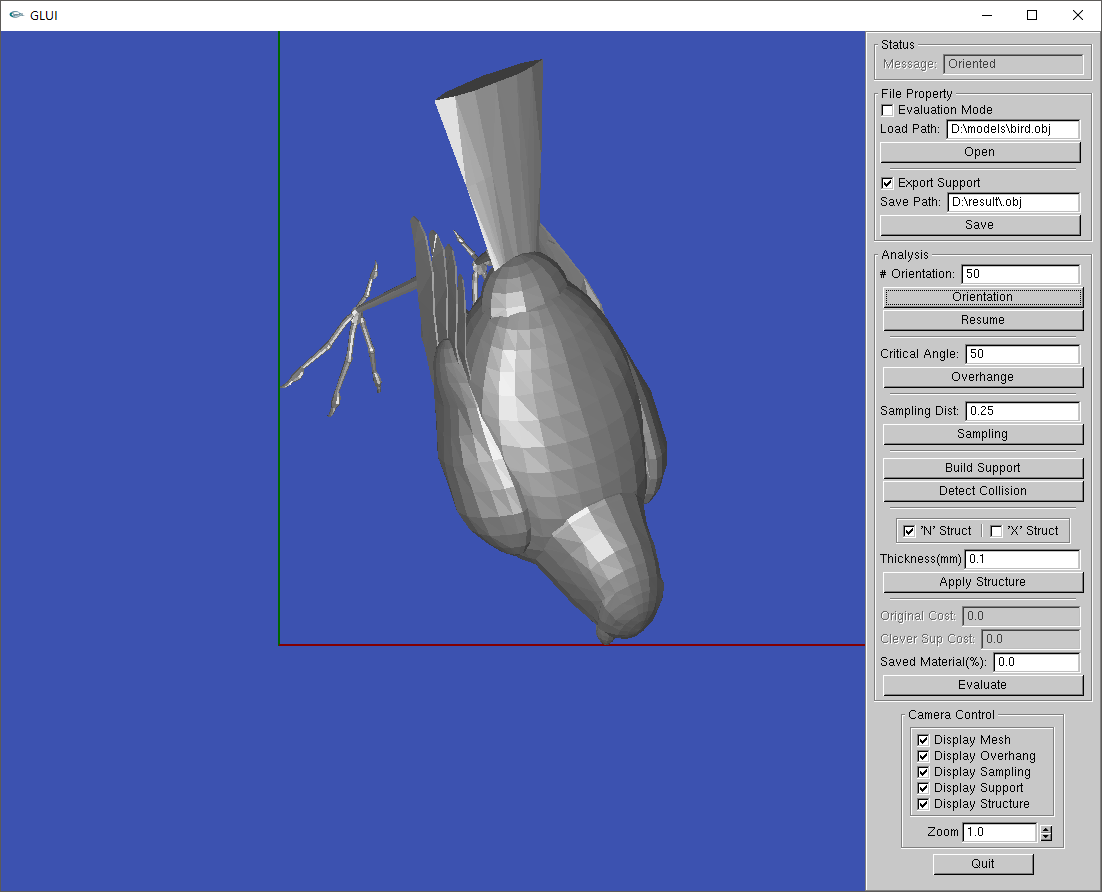
\includegraphics[width=1.0\textwidth]{orientation.png}
  	\caption{\textit{Input the number of random rotations, the model will be rotated into the best orientation with least overhanging points. User can resume the model by clicking the "resume" button.}}
	\end{figure}
	\section{Overhang}
	\begin{figure}[H]
  		\centering
      	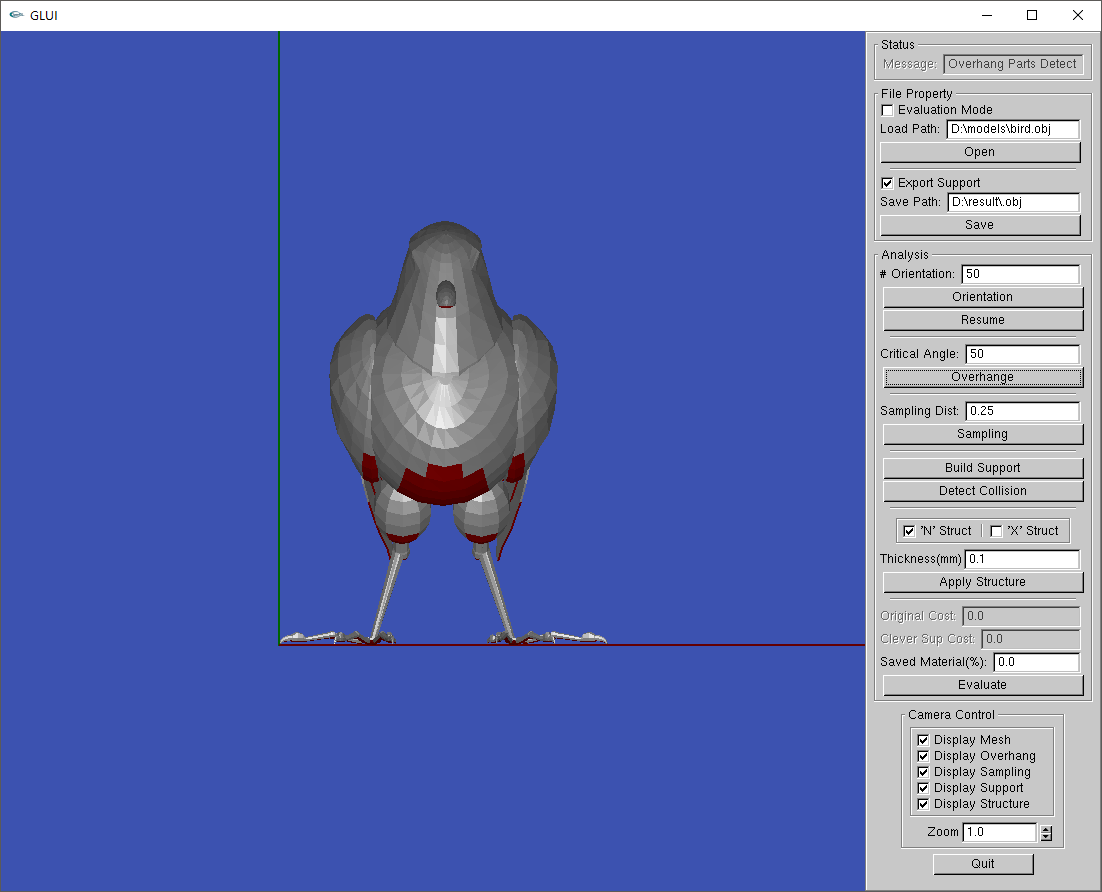
\includegraphics[width=1.0\textwidth]{overhang.png}
  	\caption{\textit{Input the critical angle of the 3D printer, the overhang parts will be colored red.}}
	\end{figure}
	\section{Sampling}
	\begin{figure}[H]
  		\centering
      	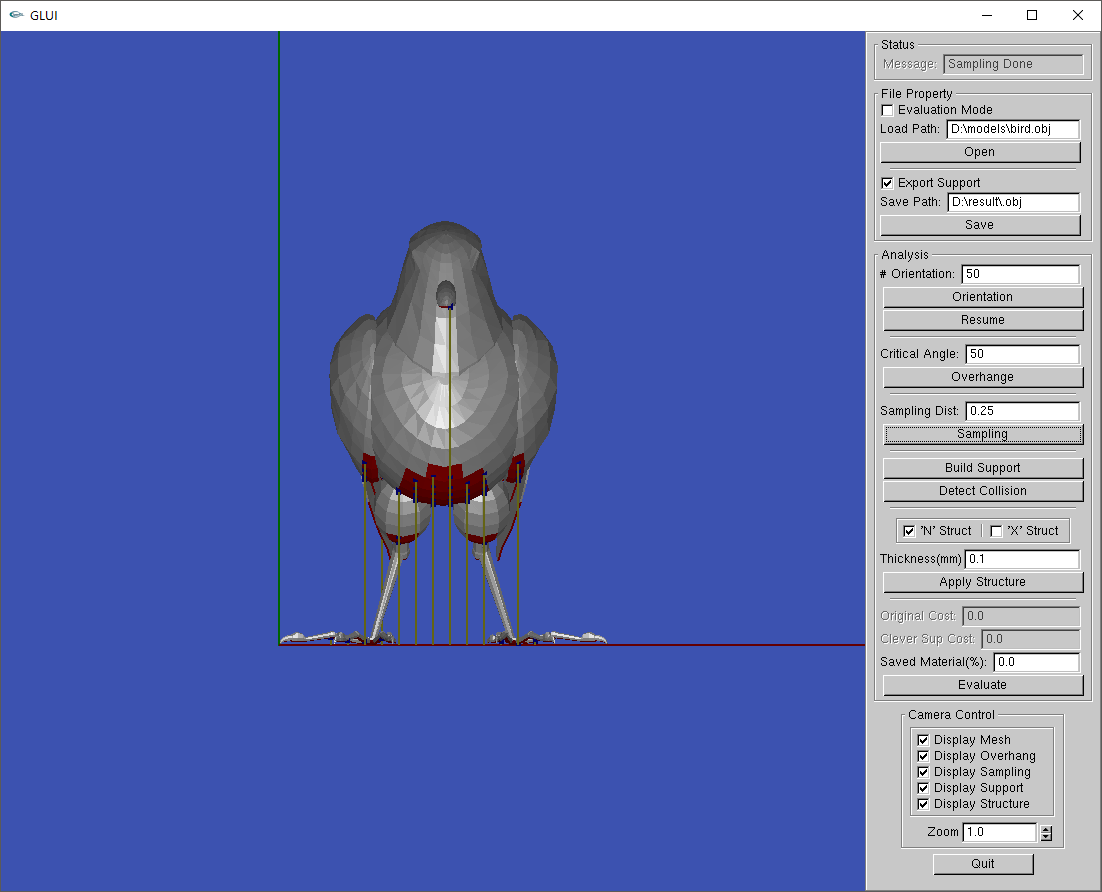
\includegraphics[width=1.0\textwidth]{sampling.png}
  	\caption{\textit{Input the sampling distance in mm. Please note that if the sampling distance is set too small, the program may crash for big models. Please set the value approately. Usually 0.1 for small models and 0.15 for big models for the minimum value supported.}}
	\end{figure}
	\section{Build Tree}
	\begin{figure}[H]
  		\centering
      	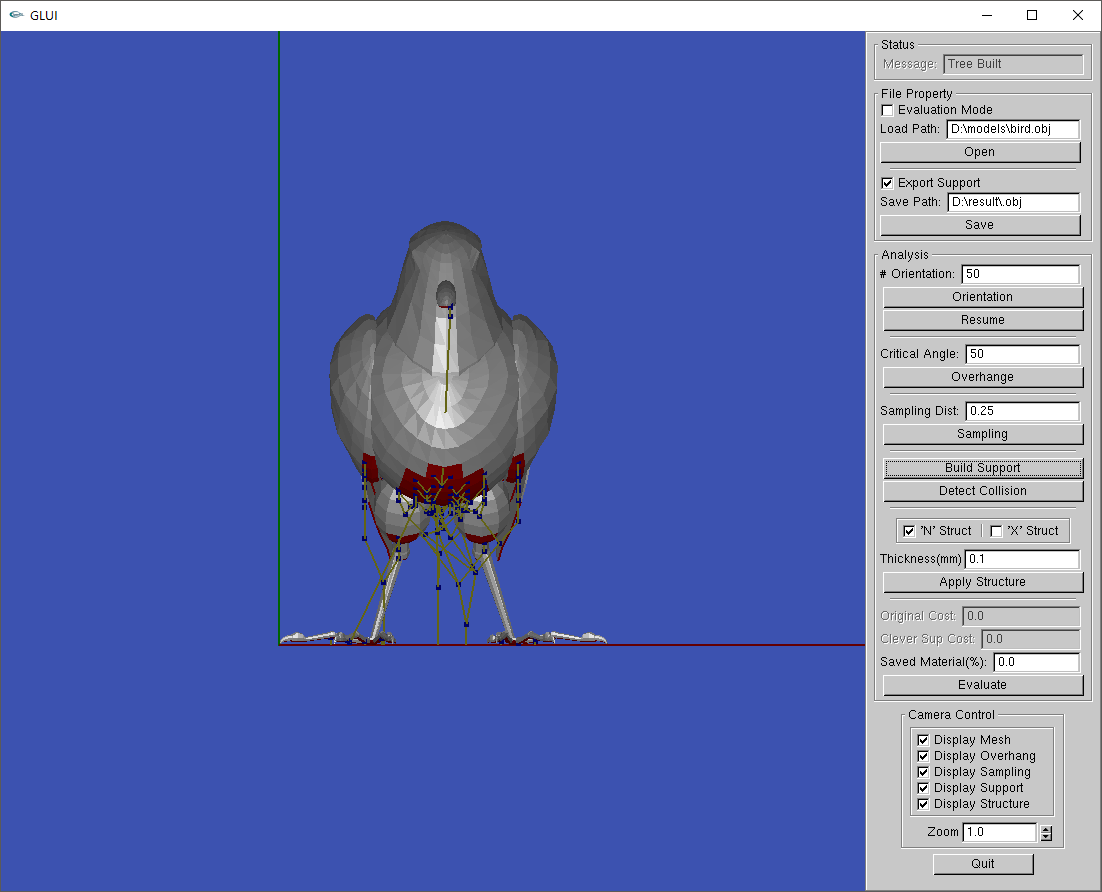
\includegraphics[width=1.0\textwidth]{build.png}
  	\caption{\textit{Click the "Build Support" button, and the support tree will be shown.The blue points are the overhanging points.}}
	\end{figure}
	\section{Detection}
	\begin{figure}[H]
  		\centering
      	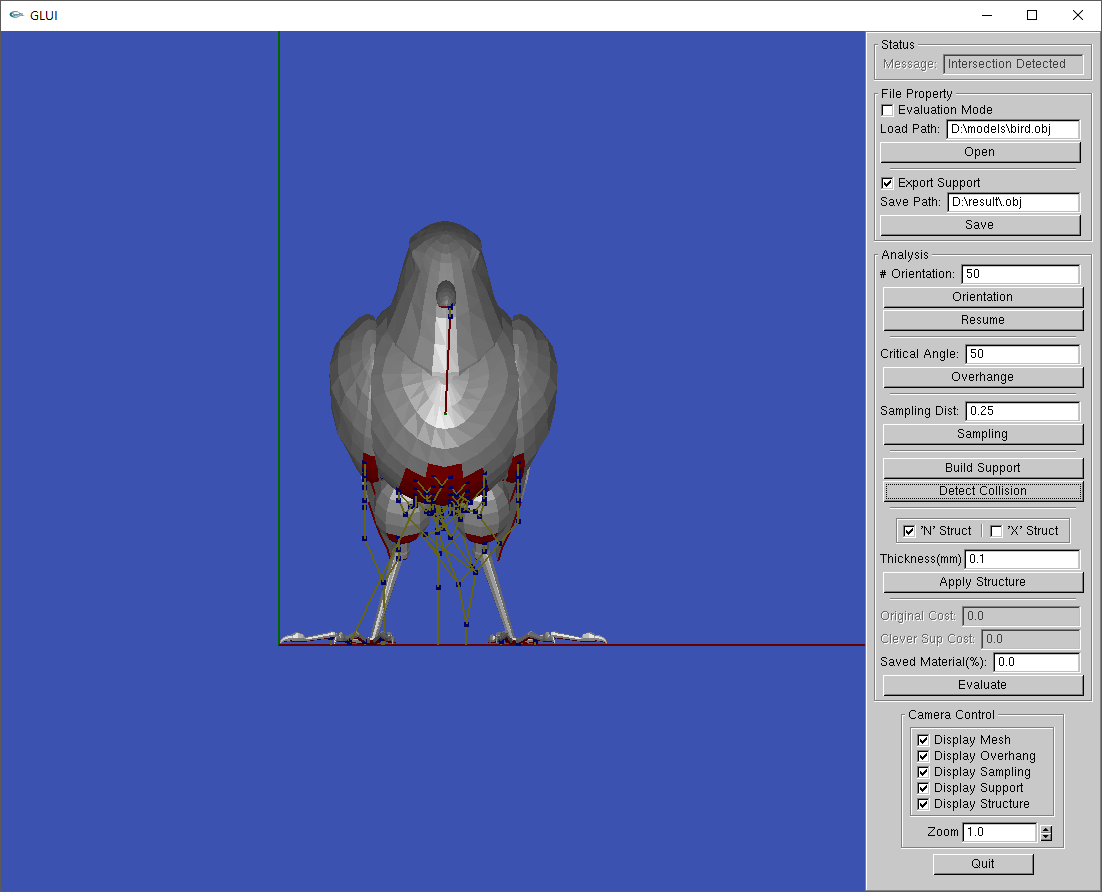
\includegraphics[width=1.0\textwidth]{collision.png}
  	\caption{\textit{Click the "Detec Collision" button, the tree branches which have intersection with the mesh will be modified. The new branches will be shown in red.}}
	\end{figure}
	\section{Structure}
	\begin{figure}[H]
  		\centering
      	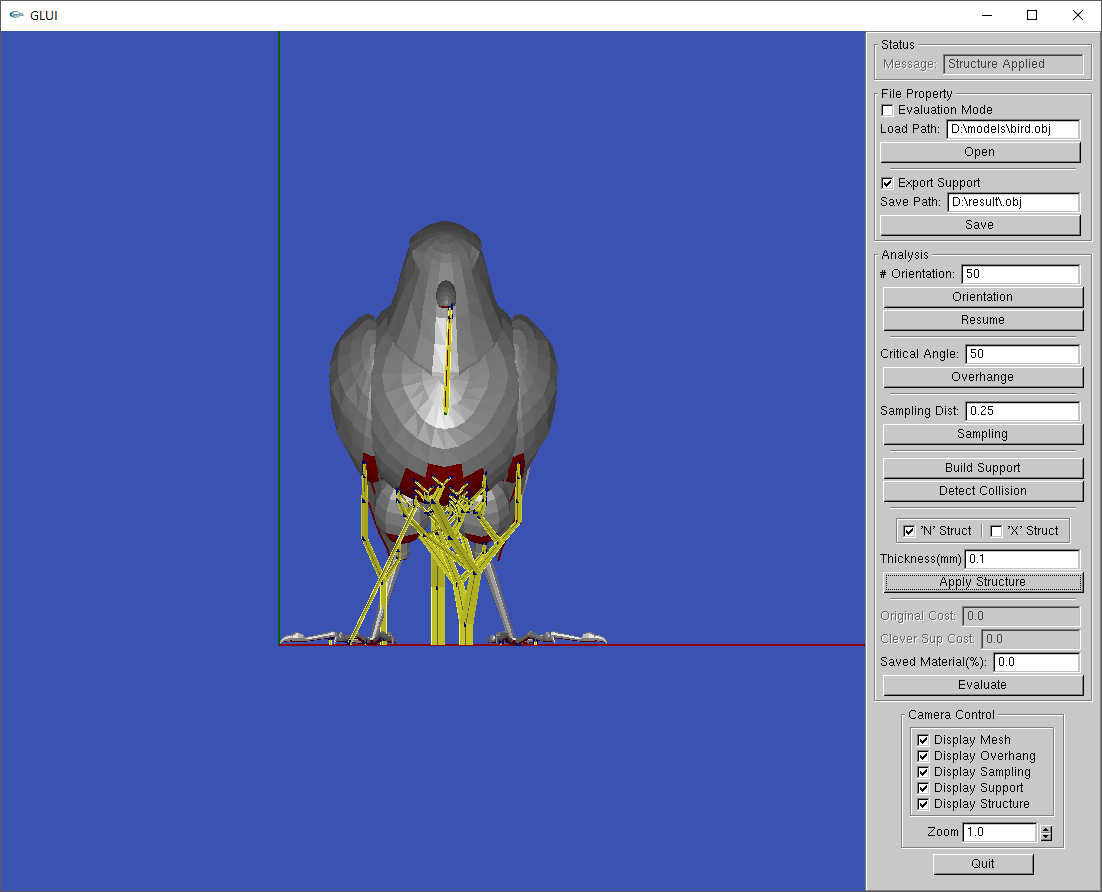
\includegraphics[width=1.0\textwidth]{structure.png}
  	\caption{\textit{Select the type of the structure first, and then input the thickness of the support. Please make sure the value ranges from 0.05 to 0.6mm, otherwise there will be display error.}}
	\end{figure}
	\section{Evaluation}
	\begin{figure}[H]
  		\centering
      	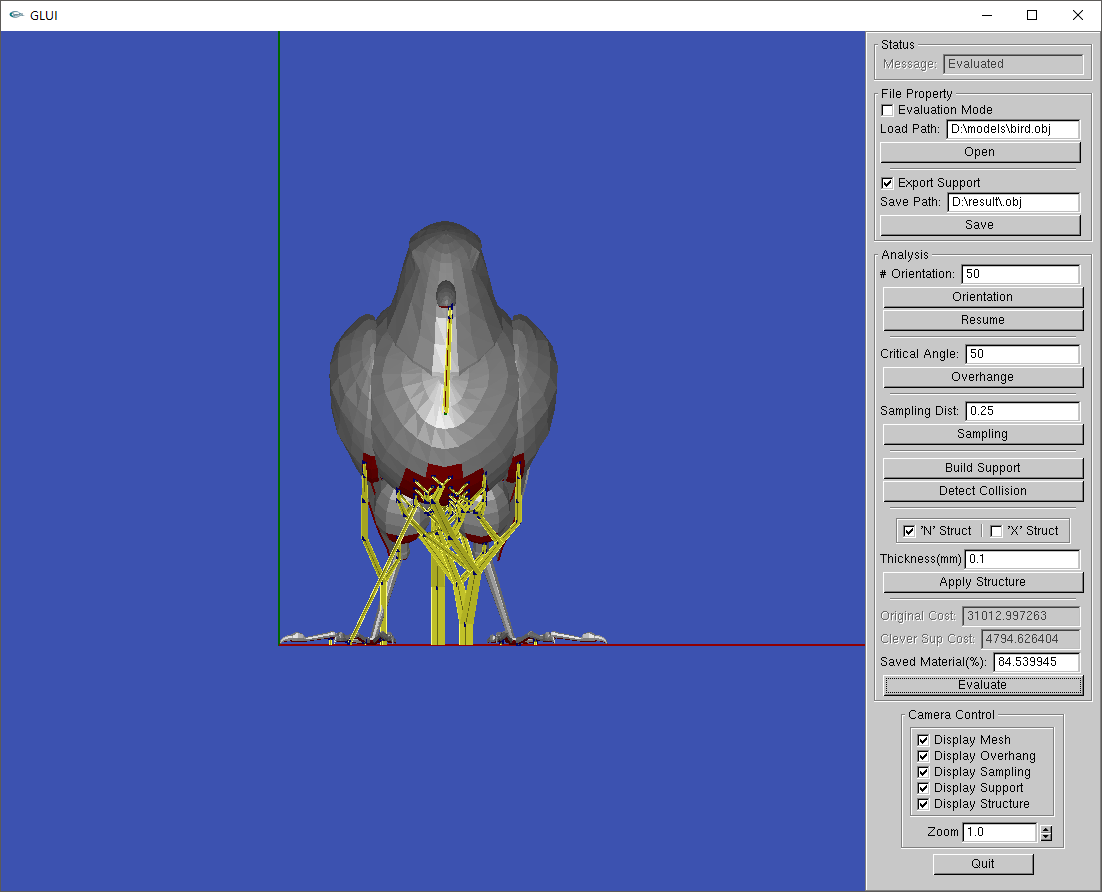
\includegraphics[width=1.0\textwidth]{evaluate.png}
  	\caption{\textit{Click "Evaluate" button, and the total amoun of the supporting face area will be shown.}}
	\end{figure}
	\section{Display Control}
	\begin{figure}[H]
  		\centering
      	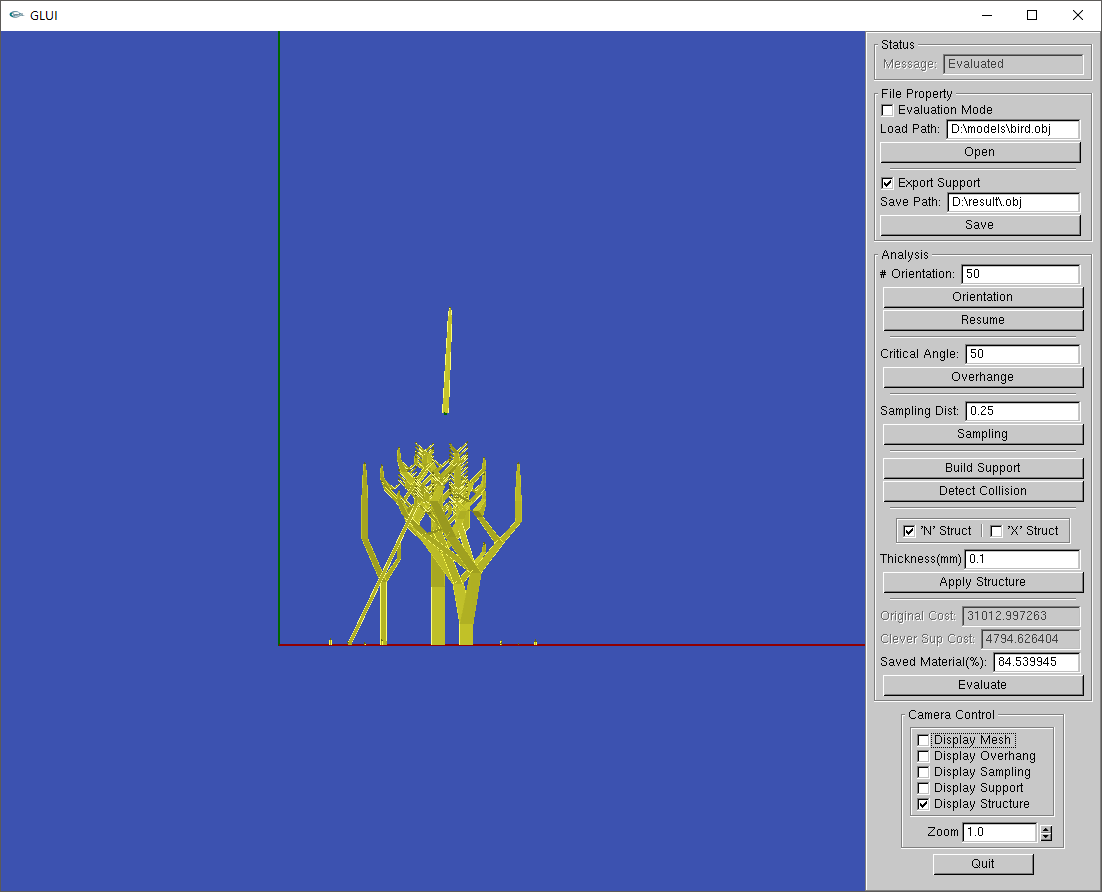
\includegraphics[width=1.0\textwidth]{control.png}
  	\caption{\textit{Select different parts of the model to be displayed. Here only the support structure is display.}}
	\end{figure}
\end{document}